  \subsection[Stockage]{Stockage : block, objet, SDS}

  \begin{frame}
    \frametitle{Stockage block}
     \begin{itemize}
      \item Accès à des raw devices type \textit{/dev/vdb}
      \item Possibilité d'utiliser n'importe quel système de fichiers
      \item Compatible avec toutes les applications legacy
     \end{itemize}
   \end{frame}

   \begin{frame}
    \frametitle{Stockage objet}
      \item Pousser et retirer des objets dans un container/bucket
      \item Pas de hiérarchie des données, pas de système de fichiers
      \item Accès par les APIs
      \item L'application doit être conçue pour tirer partie du stockage objet
     \end{itemize}
   \end{frame}

   \begin{frame}
    \frametitle{Stockage objet : schéma}
    \begin{center}
      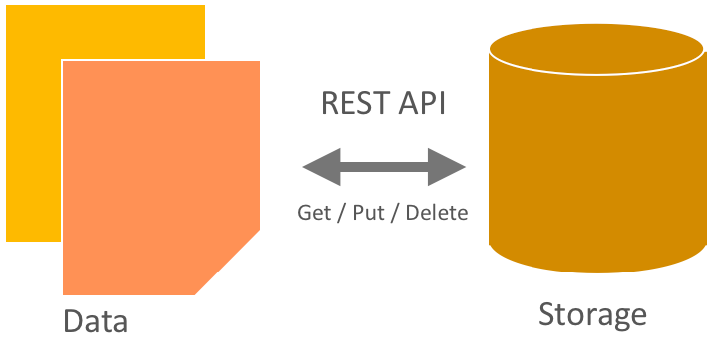
\includegraphics{images/stockage-objet.png}
    \end{center}
  \end{frame}

  \begin{frame}
    \frametitle{SDS : Software Defined Storage}
      \item Utilisation de commodity hardware
      \item Pas de RAID matériel
      \item Le logiciel est responsable de garantir les données
      \item Les pannes matérielles sont prises en compte et gérées
     \end{itemize}
   \end{frame}

   \begin{frame}
    \frametitle{Deux solutions : OpenStack Swift et Ceph}
     \begin{itemize}
      \item Swift fait partie du projet OpenStack et fournit du stockage objet
      \item Ceph fournit du stockage objet, block et FS
      \item Les deux sont implémentés en SDS\pause
      \item Théorème CAP : on en choisit deux
     \end{itemize}
   \end{frame}

   \begin{frame}
  \frametitle{Théorème CAP}
  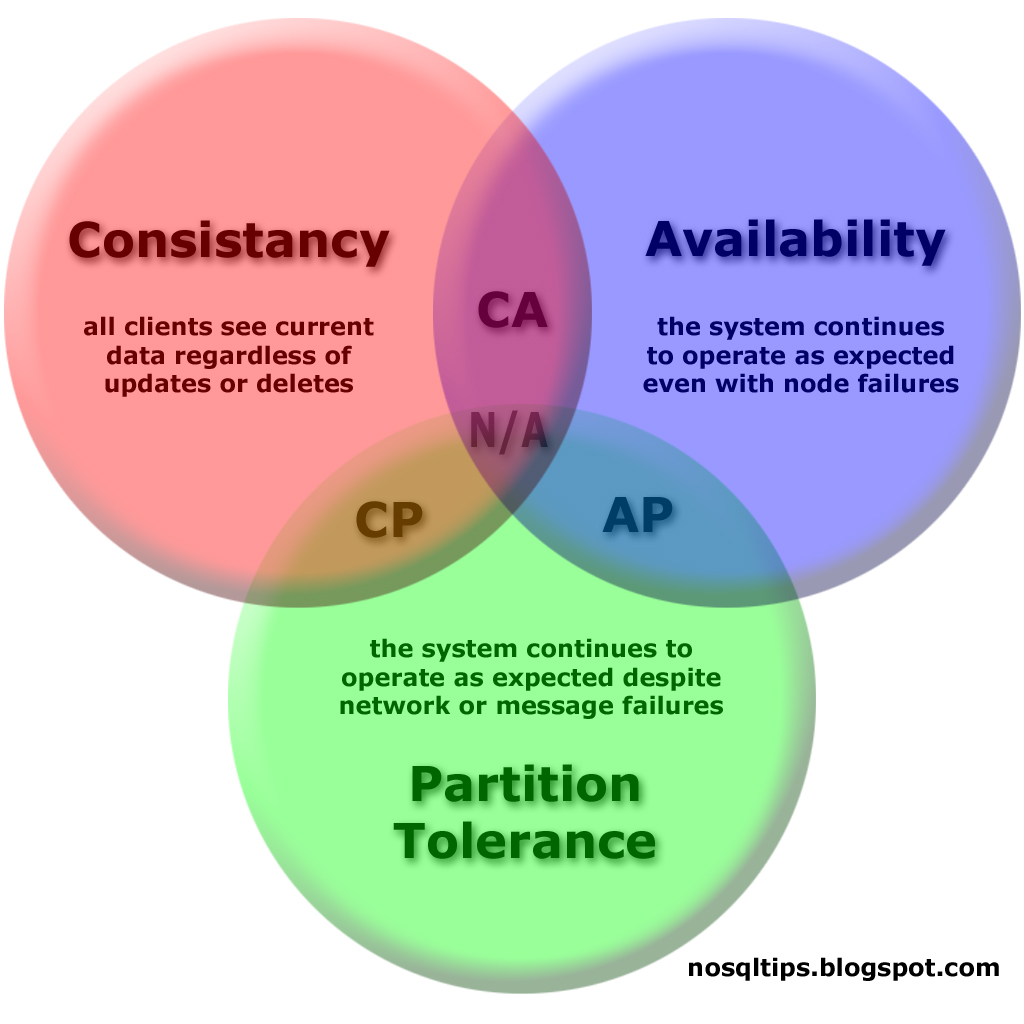
\includegraphics[width=\textwidth,height=\textheight]{images/cap.jpg}
  \end{frame}

  \begin{frame}
  \frametitle{Swift}
     \begin{itemize}
      \item Swift est un projet OpenStack
      \item Le projet est né chez Rackspace avant la création d'OpenStack
      \item Swift est en production chez Rackspace depuis lors
      \item C'est le composant le plus mature d'OpenStack
     \end{itemize}
   \end{frame}

   \begin{frame}
  \frametitle{Ceph}
    \begin{itemize}
      \item Projet totalement parallèle à OpenStack
      \item Supporté par une entreprise (Inktank) récemment rachetée par Red Hat
      \item Fournit d'abord du stockage objet
      \item L'accès aux données se fait via RADOS :
      \begin{itemize}
        \item Accès direct depuis une application avec librados
        \item Accès via une API REST grâce à radosgw
      \end{itemize}
      \item La couche RBD permet d'accéder aux données en mode block (volumes)
      \item CephFS permet un accès par un système de fichiers POSIX
    \end{itemize}
   \end{frame}

    \frametitle{Le nouveau modèle "big tent"}
    \begin{itemize}
      \item Évolutions presque totalement implémentées
      \item Objectif : résoudre les limitations du modèle incubation/intégré
      \item Inclusion {a priori} de l'ensemble de l'écosystème OpenStack
      \item \textit{Programs} $\rightarrow$ \textit{Project Teams}
      \item Disparation des statuts en incubation et intégré
      \item Utilisation de tags factuels et objectifs
    \end{itemize}
  \end{frame}

  \begin{frame}
    \frametitle{Traduction}
    \begin{itemize}
      \item La question de la traduction est dorénavant prise en compte (officialisation de l'équipe \textit{i18n})
      \item Seules certaines parties sont traduites, comme Horizon
      \item La traduction française est aujourd'hui une des plus avancées
      \item Utilisation de la plateforme Transifex (en cours de migration vers l'outil libre Zanata)
    \end{itemize}
  \end{frame}

    \frametitle{Stackforge}
    \begin{itemize}
      \item Forge pour les nouveaux projets en lien avec OpenStack
      \item Ils bénéficient de l'infrastructure du projet OpenStack, mais la séparation reste claire
      \item Les projets démarrent dans Stackforge et peuvent ensuite rejoindre le projet OpenStack
      \item En train de disparaitre au profit du modèle "big tent"
    \end{itemize}
  \end{frame}

  \begin{frame}
    \frametitle{Implémentation}
    \begin{itemize}
      \item Chaque sous-projet est découpé en plusieurs services\pause
      \item Communication entre les services : AMQP (RabbitMQ)\pause
      \item Base de données : relationnelle SQL (MySQL/MariaDB)\pause
      \item Réseau : OpenVSwitch\pause
      \item En général : réutilisation de composants existants\pause
      \item Tout est développé en Python (Django pour la partie web)\pause
      \item APIs supportées : OpenStack et équivalent Amazon\pause
      \item Multi tenancy
    \end{itemize}
  \end{frame}

   \begin{frame}
    \frametitle{Architecture}
    \begin{center}
      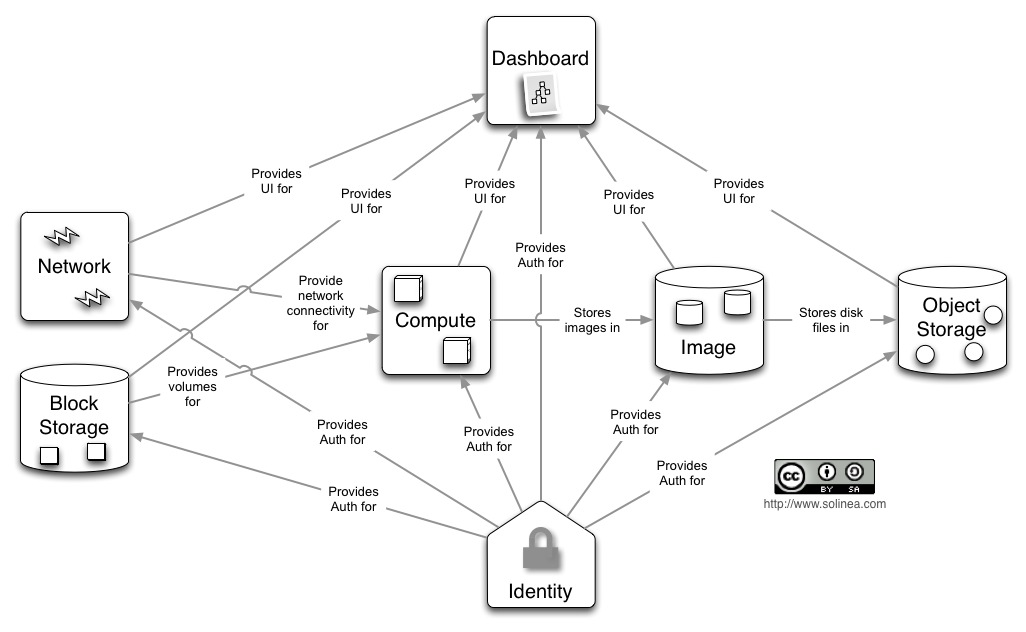
\includegraphics[width=\textwidth]{images/architecture-simple.jpg}
    \end{center}
  \end{frame}

   \begin{frame}
    \frametitle{Cycle de développement : 6 mois}
    \begin{itemize}
      \item Le planning est publié, exemple : \url{https://wiki.openstack.org/wiki/Mitaka_Release_Schedule}
      \item Milestone releases
      \item Freezes : FeatureProposal, Feature, String
      \item RC releases
      \item Stable releases
      \item Ce modèle de cycle de développement a évolué depuis le début du projet
      \item Cas particulier de Swift et de plus en plus de composants
      \item Depuis Liberty, chaque composant gère son propre versionnement
    \end{itemize}
  \end{frame}

  \begin{frame}
    \frametitle{Versionnement depuis Liberty}
    \begin{itemize}
      \item \textit{Semantic versioning}
      \item Chaque projet est indépendant
      \item Dans le cadre du cycle de release néanmoins
      \item \url{http://docs.openstack.org/releases/}
    \end{itemize}
  \end{frame}

  \begin{frame}
    \frametitle{Où trouver des informations sur le développement d'OpenStack}
    \begin{itemize}
      \item Principalement sur le wiki : \url{https://wiki.openstack.org}
      \item Les blueprints et bugs sur Launchpad/StoryBoard : \url{https://launchpad.net/openstack}, \url{https://storyboard.openstack.org}, \url{http://specs.openstack.org/}
      \item Les patchs proposés et leurs reviews sont sur Gerrit : \url{https://review.openstack.org}
      \item L'état de la CI (entre autres) : \url{http://status.openstack.org}
      \item Le code est disponible dans Git : \url{https://git.openstack.org}
      \item Les sources (tarballs) sont disponibles : \url{http://tarballs.openstack.org/}
    \end{itemize}
  \end{frame}

  \begin{frame}
    \frametitle{Qui contribue ?}
    \begin{itemize}
      \item \textit{Active Technical Contributor}
      \item ATC : personne ayant au moins une contribution récente dans un projet OpenStack reconnu
      \item Les ATC sont invités aux summits et ont le droit de vote
      \item \textit{Core reviewer} : ATC ayant les droits pour valider les patchs dans un projet
      \item \textit{Project Team Lead} (PTL) : élu par les ATCs de chaque projet
      \item Stackalytics fournit des statistiques sur les contributions
    \end{itemize}
    \url{http://stackalytics.com/}
  \end{frame}

  \begin{frame}
    \frametitle{OpenStack Summit}
    \begin{itemize}
      \item Aux USA jusqu'en 2013
      \item Aujourd'hui : alternance Amérique de Nord et Asie/Europe
      \item Quelques centaines au début à 4500 participants aujourd'hui
      \item En parallèle : conférence (utilisateurs, décideurs) et Design Summit (développeurs)
      \item Détermine le nom de la release : lieu/ville à proximité du Summit
      \item \textit{Upstream Training}
    \end{itemize}
  \end{frame}

  \begin{frame}
    \frametitle{Exemple du Summit d'avril 2013 à Portland}
    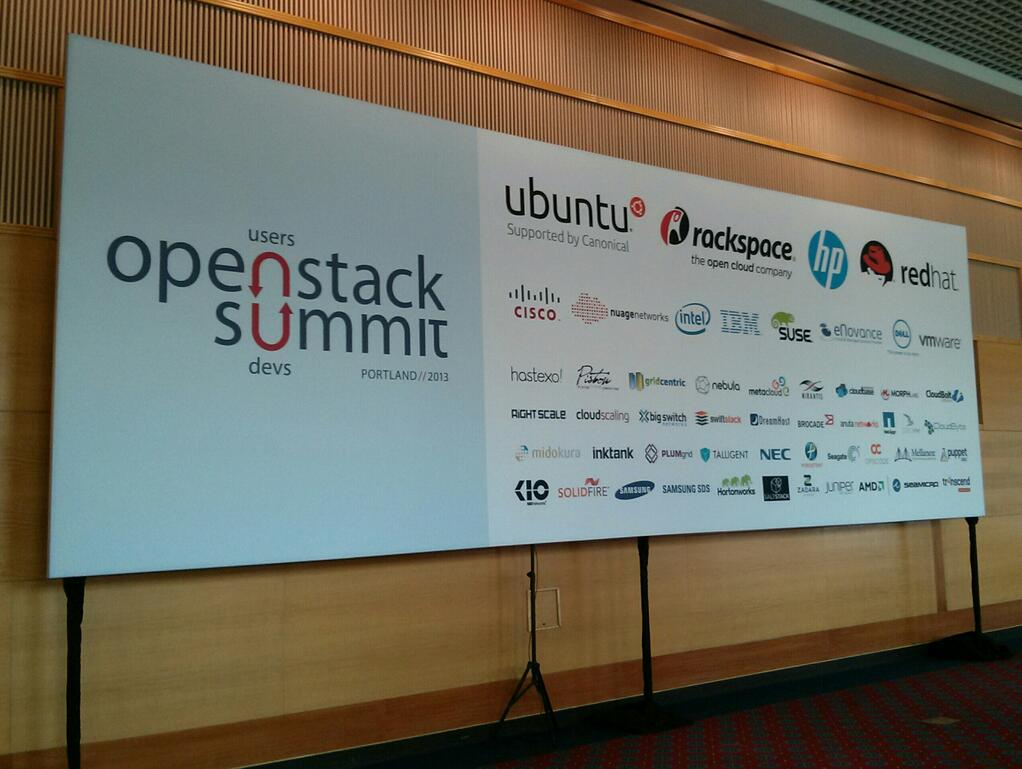
\includegraphics[width=\textwidth]{images/photo-summit.jpg}
  \end{frame}

  \begin{frame}
    \frametitle{Exemple du Summit d'octobre 2015 à Tokyo}
    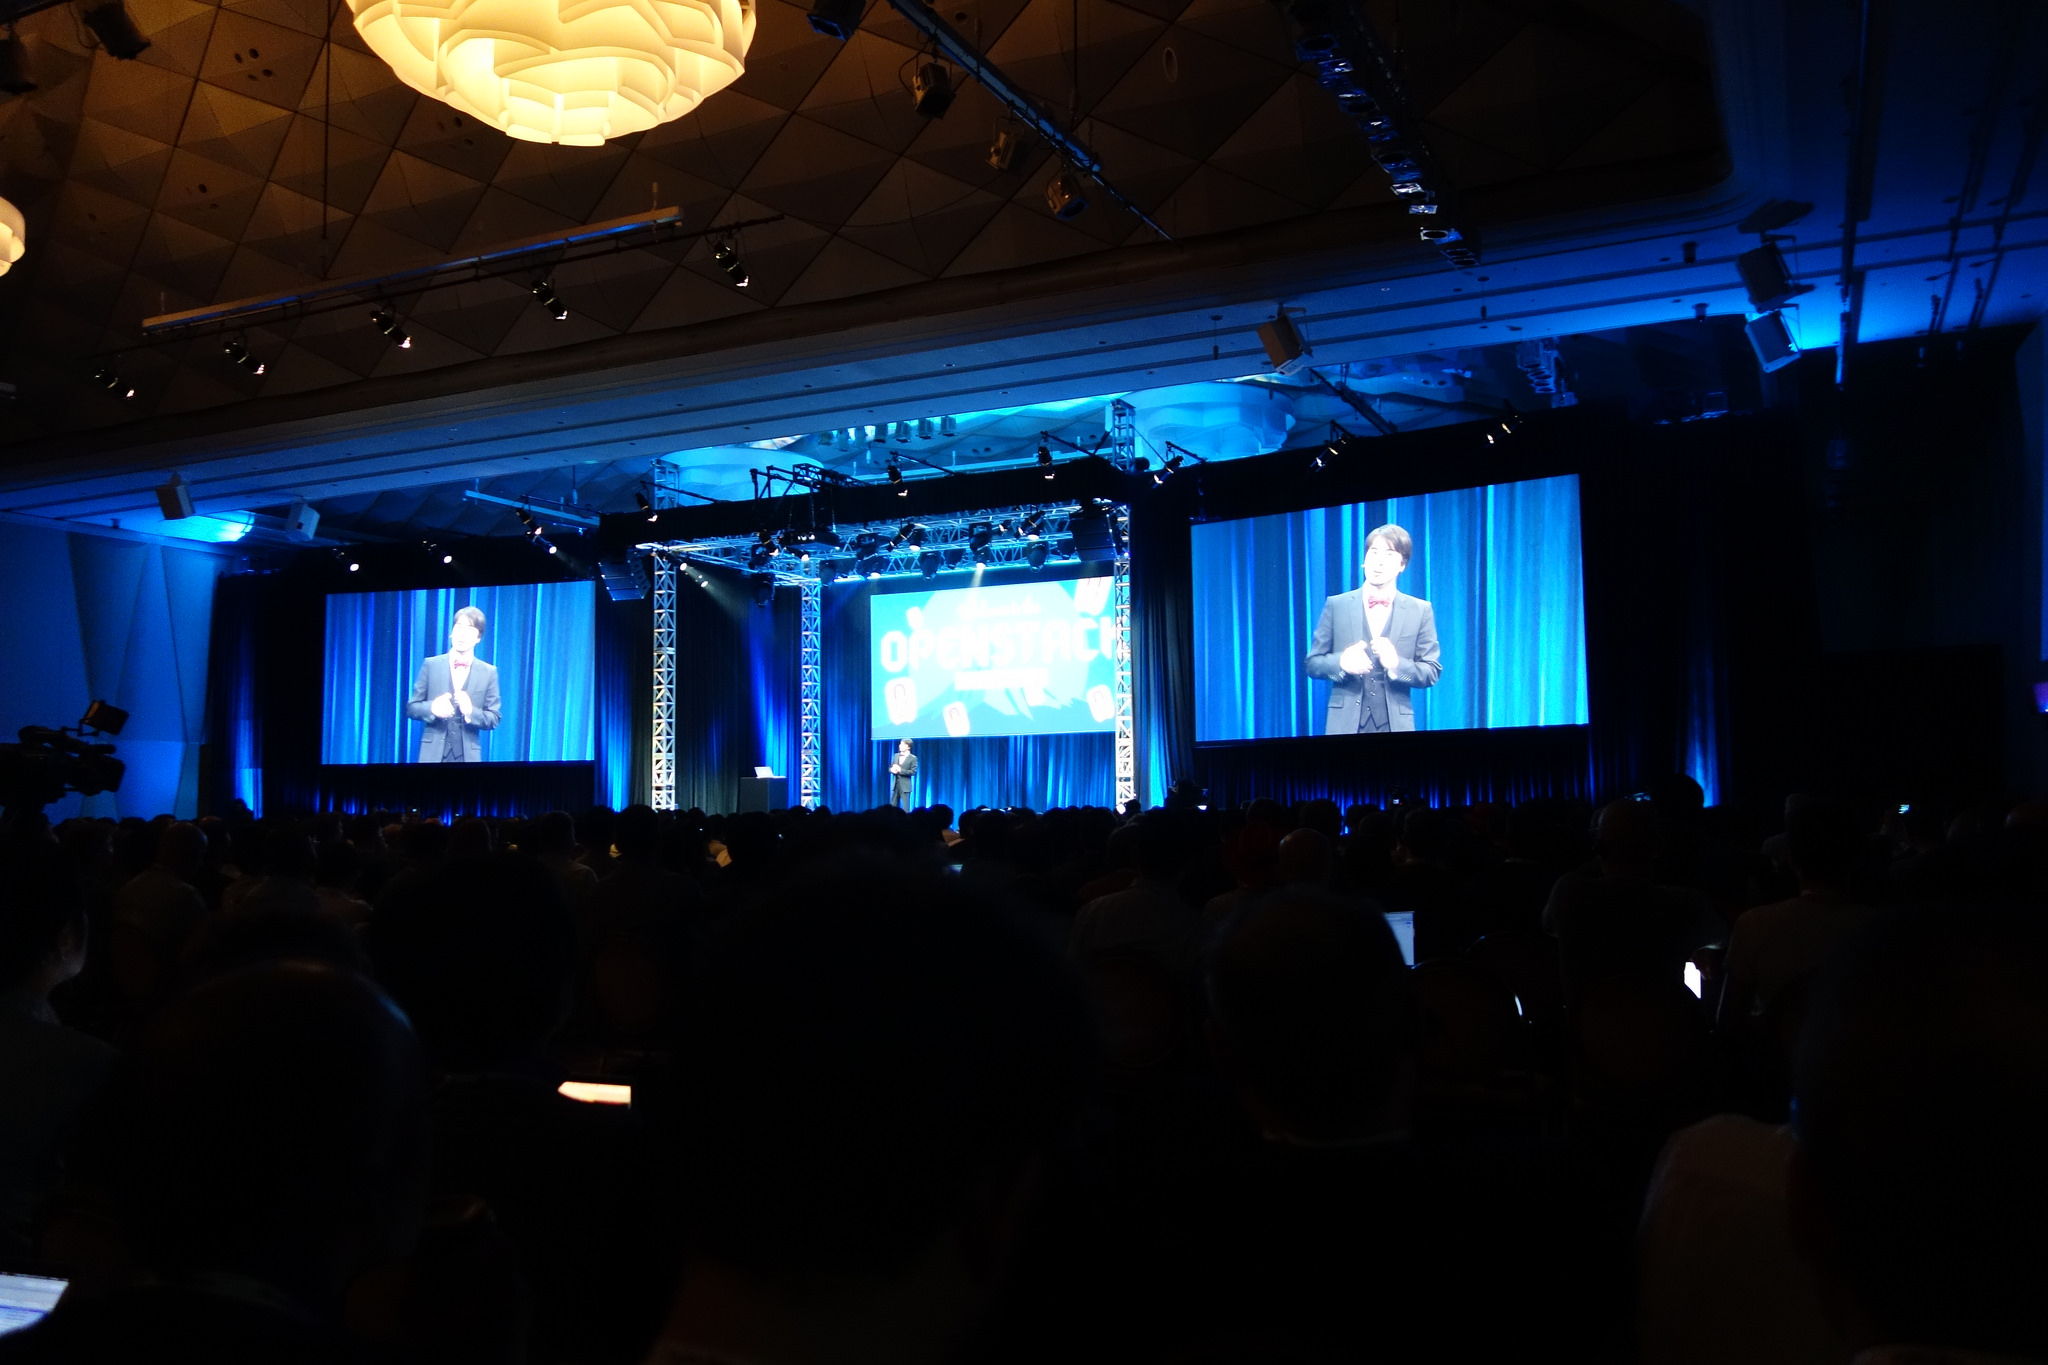
\includegraphics[width=\textwidth]{images/photo-summit1.jpg}
    Photo : Elizabeth K. Joseph, CC BY 2.0, Flickr/pleia2
  \end{frame}

  \begin{frame}
    \frametitle{Exemple du Summit d'octobre 2015 à Tokyo}
    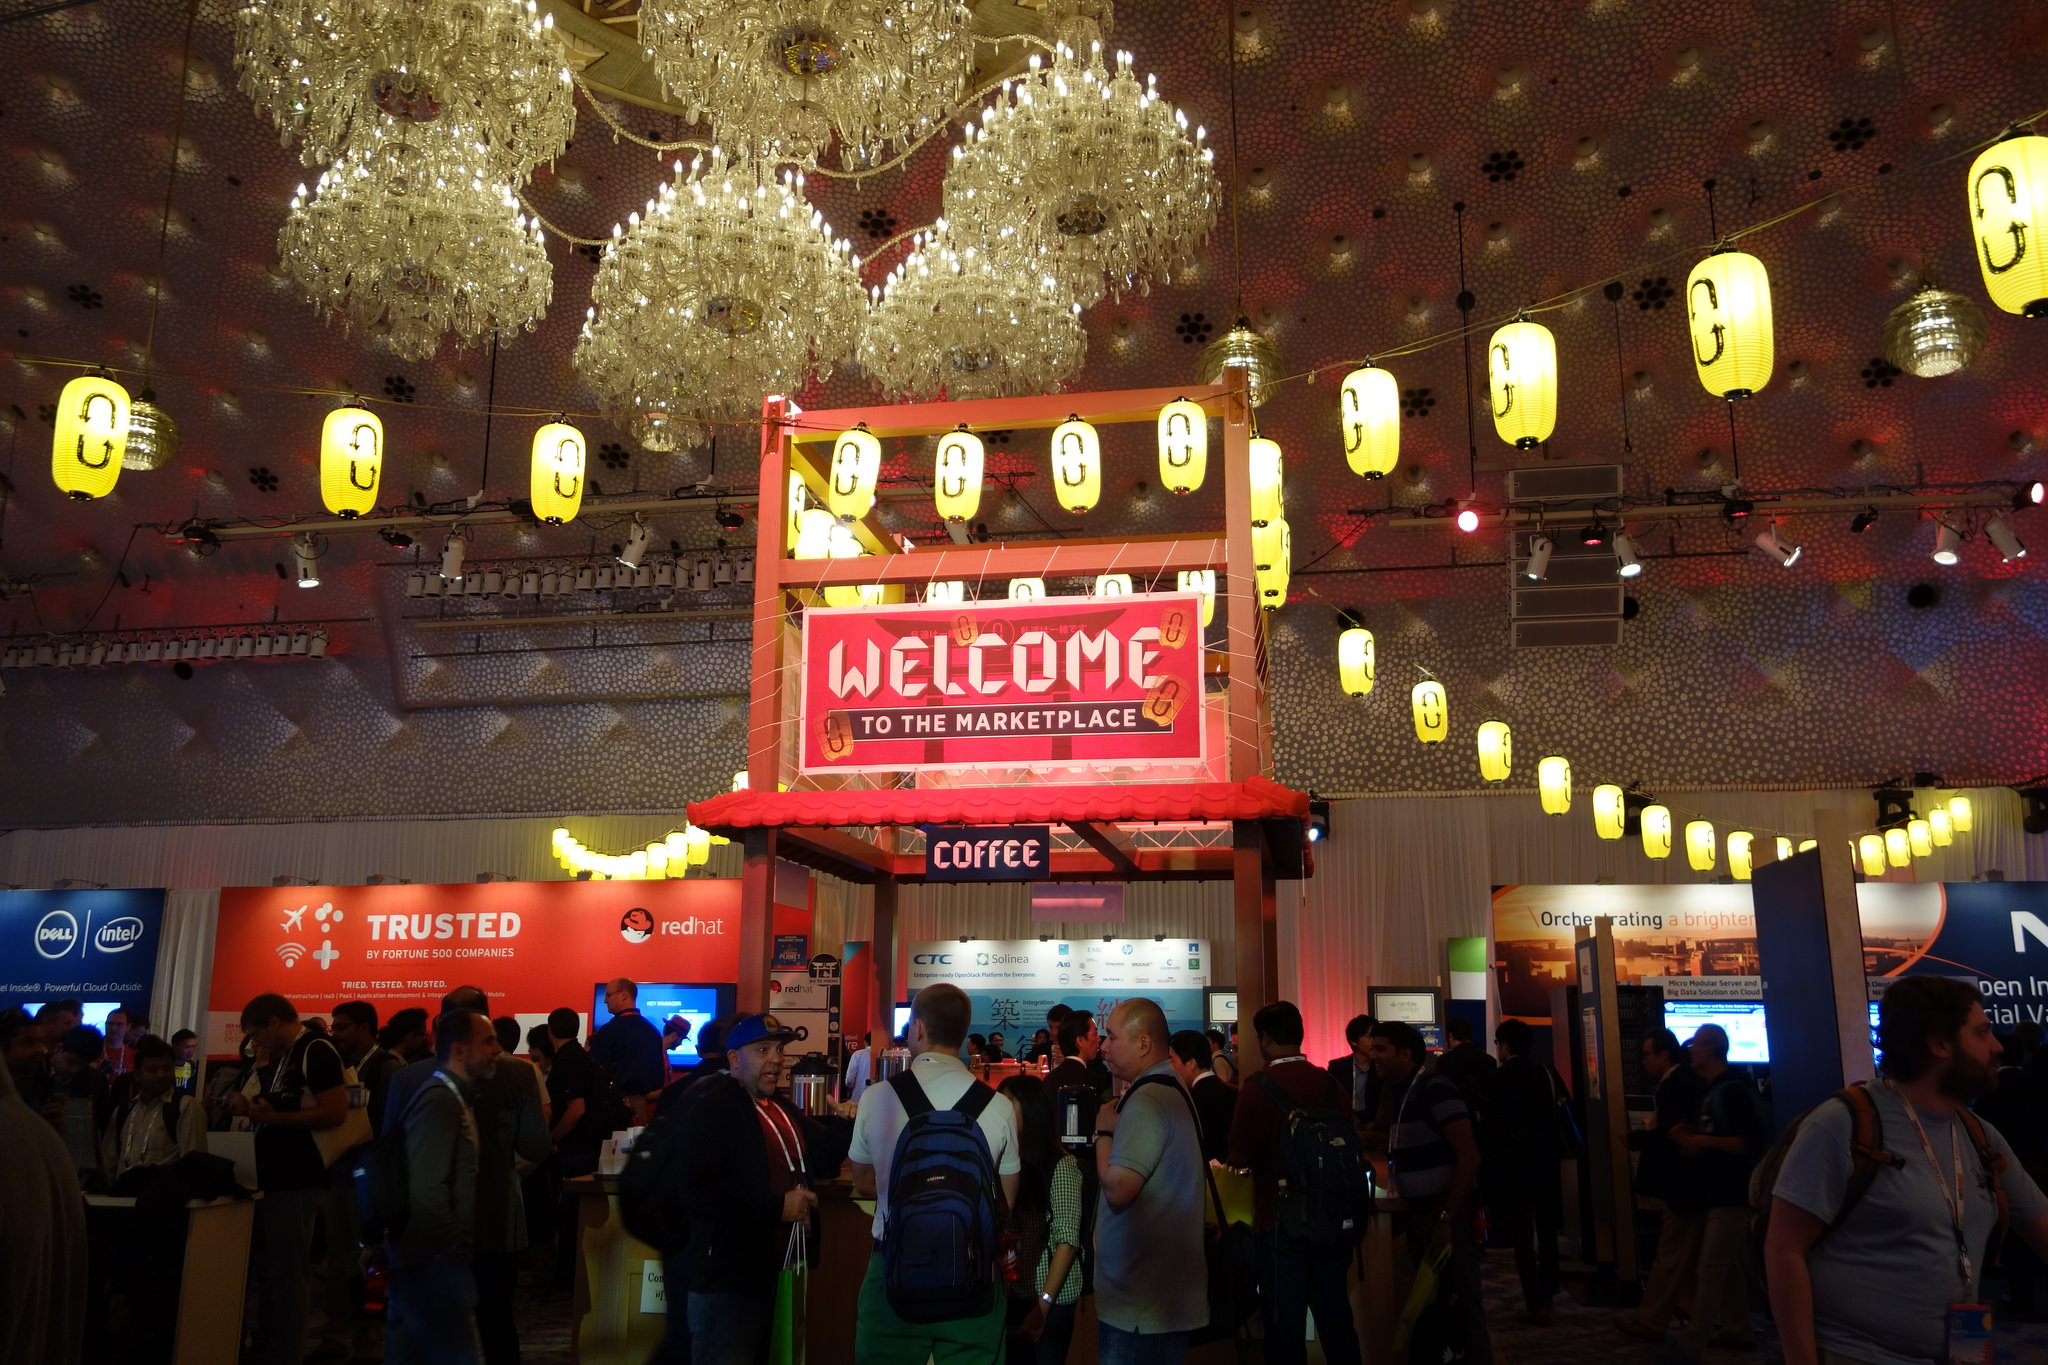
\includegraphics[width=\textwidth]{images/photo-summit2.jpg}
    Photo : Elizabeth K. Joseph, CC BY 2.0, Flickr/pleia2
  \end{frame}

  \begin{frame}
    \frametitle{Exemple du Summit d'octobre 2015 à Tokyo}
    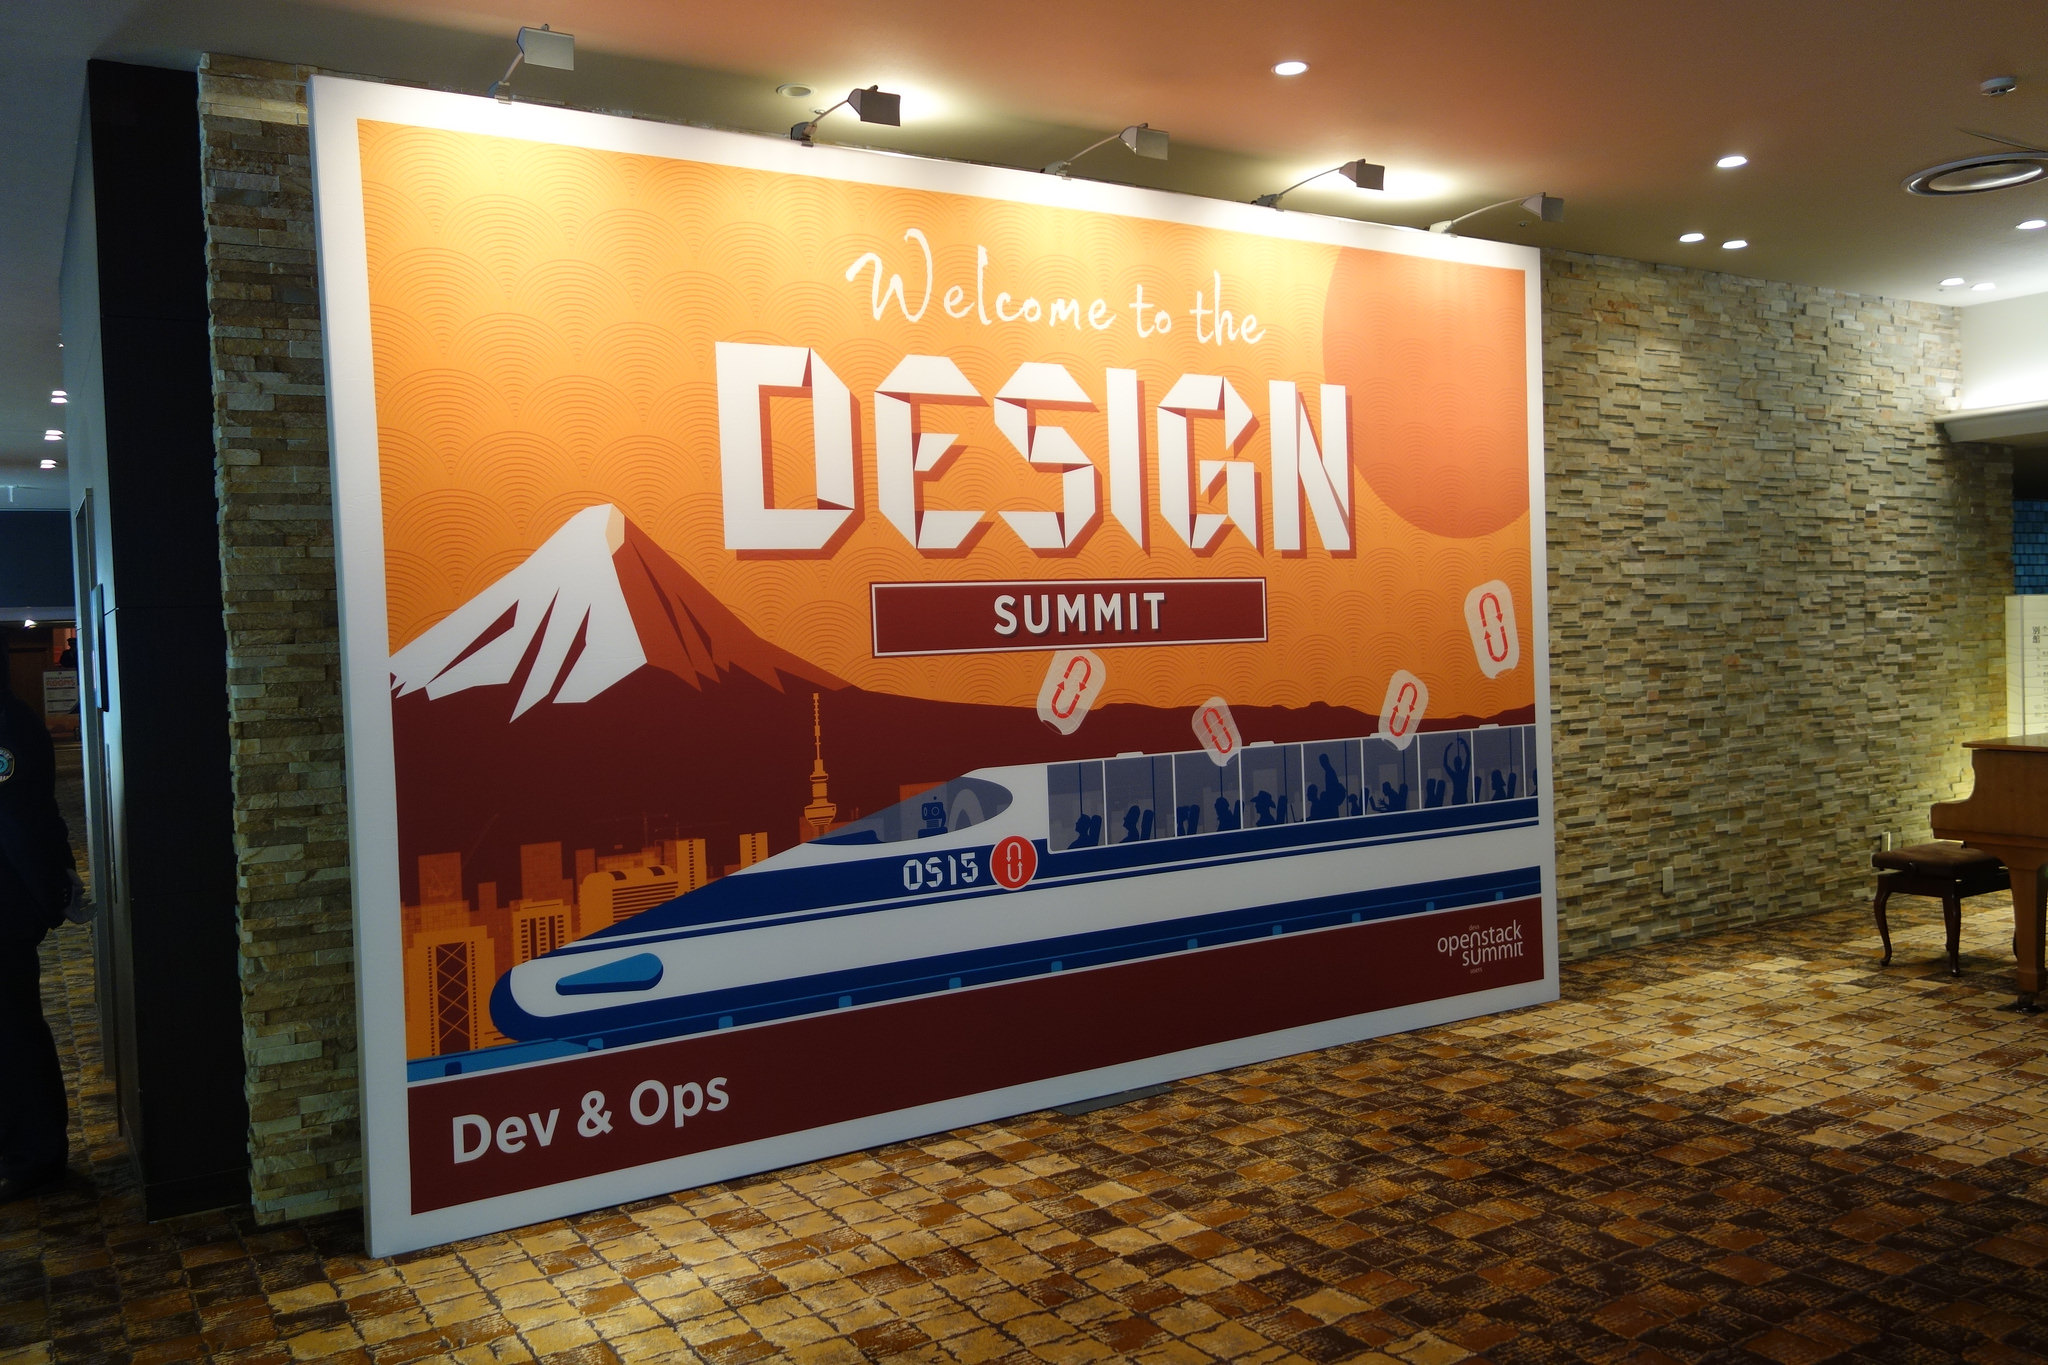
\includegraphics[width=\textwidth]{images/photo-summit3.jpg}
    Photo : Elizabeth K. Joseph, CC BY 2.0, Flickr/pleia2
  \end{frame}

  \begin{frame}
    \frametitle{Exemple du Summit d'octobre 2015 à Tokyo}
    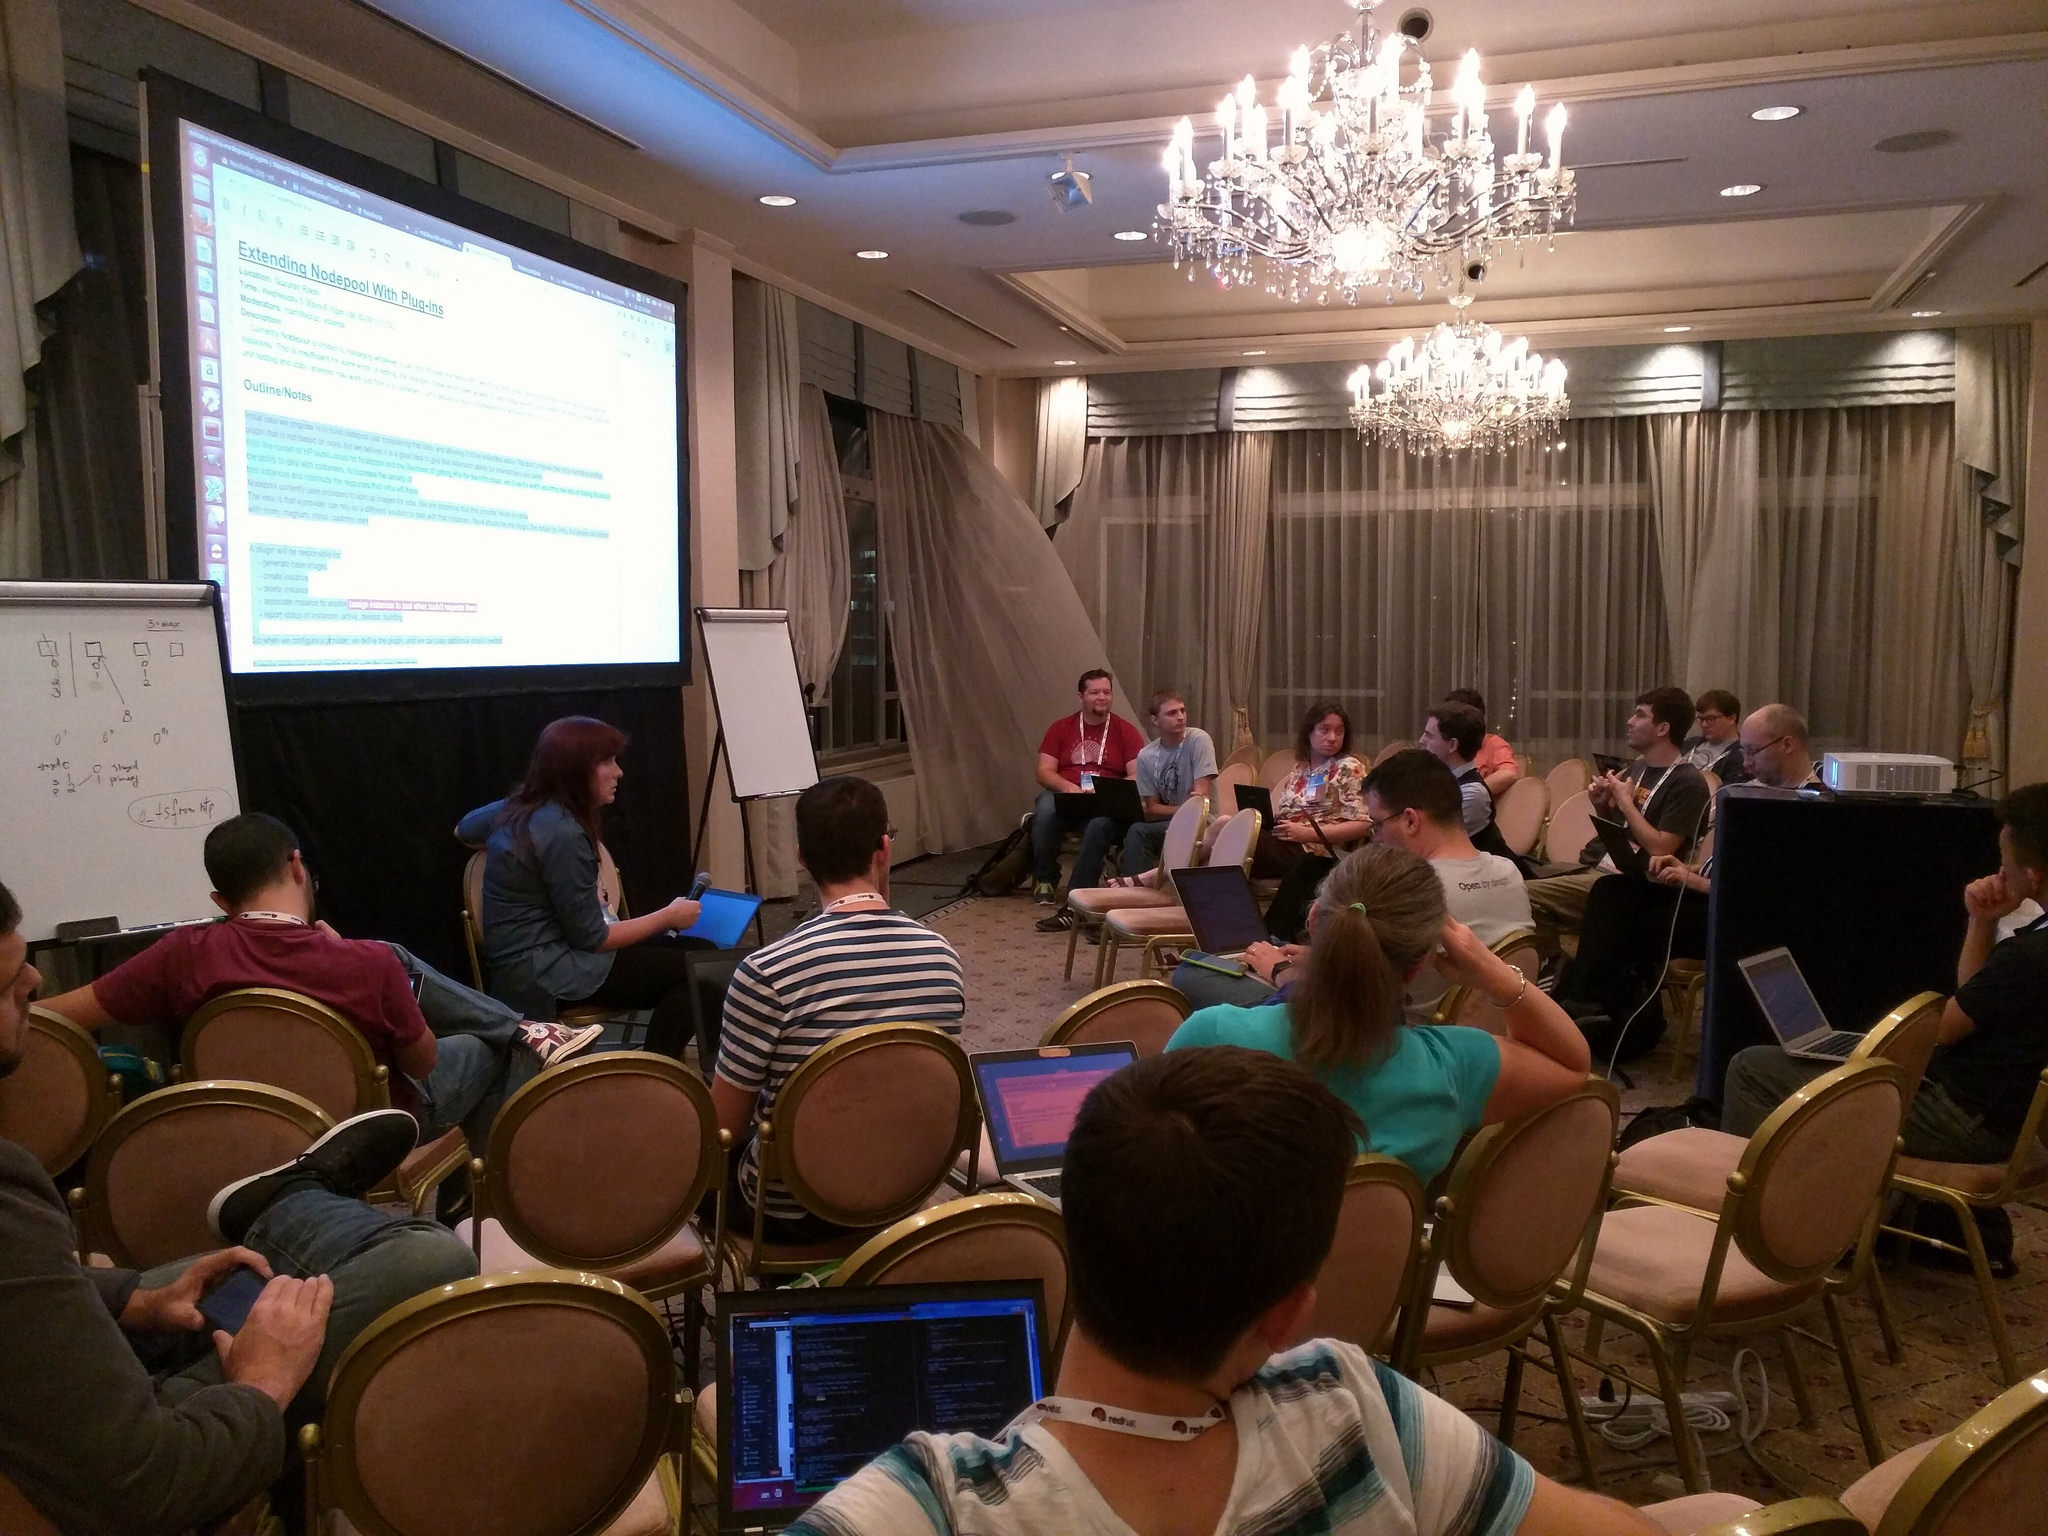
\includegraphics[width=\textwidth]{images/photo-summit4.jpg}
    Photo : Elizabeth K. Joseph, CC BY 2.0, Flickr/pleia2
  \end{frame}

   \begin{frame}
    \frametitle{Développement du projet : en détails}
    \begin{itemize}
      \item Ouvert à tous (individuels et entreprises)\pause
      \item Cycle de développement de 6 mois débuté par un (design) summit\pause
      \item Outils : Launchpad $\rightarrow$ Storyboard (blueprints, bugs) + Git + GitHub (code)\pause
      \item Sur chaque patch proposé :
      \begin{itemize}
        \item Revue de code (peer review) : Gerrit, \url{https://review.openstack.org}
        \item Intégration continue (continous integration) : Jenkins, Zuul, etc., \url{http://zuul.openstack.org/}
      \end{itemize}\pause
      \item Développement hyper actif : 17000 commits dans Icehouse (+25\%)\pause
      \item Fin 2012, création d'une entité indépendante de gouvernance : la fondation OpenStack
    \end{itemize}
  \end{frame}

  \begin{frame}
    \frametitle{OpenStack Infra}
    \begin{itemize}
      \item Équipe projet en charge de l'infrastructure de développement d'OpenStack
      \item Travaille comme les équipes de dev d'OpenStack et utilise les mêmes outils
      \item Résultat : une infrastructure entièrement open source et développée comme tel
    \end{itemize}
  \end{frame}

  \subsection[Orchestration]{Orchestrer les ressources de son IaaS}

  \begin{frame}
    \frametitle{Pourquoi orchestrer}
    \begin{itemize}
      \item Définir tout une infrastructure dans un seul fichier texte
      \item Être en capacité d'instancier une infrastructure entière en un appel API
      \item Autoscaling
      \begin{itemize}
        \item Adapter ses ressources en fonction de ses besoins en temps réel
        \item Fonctionnalité incluse dans le composant d'orchestration d'OpenStack
      \end{itemize}
    \end{itemize}
  \end{frame}

  \subsection[DevStack]{DevStack : faire tourner rapidement un OpenStack}

  \begin{frame}
    \frametitle{Utilité de DevStack}
    \begin{itemize}
      \item Déployer rapidement un OpenStack
      \item Utilisé par les développeurs pour tester leurs changements
      \item Utilisé pour faire des démonstrations
      \item Utilisé pour tester les APIs sans se préoccuper du déploiement
      \item Ne doit PAS être utilisé pour de la production
    \end{itemize}
  \end{frame}

  \begin{frame}
    \frametitle{Fonctionnement de DevStack}
    \begin{itemize}
      \item Un script shell qui fait tout le travail : stack.sh
      \item Un fichier de configuration : local.conf
      \item Installe toutes les dépendances nécessaires (paquets)
      \item Clone les dépôts git (branche master par défaut)
      \item Lance tous les composants dans un screen
    \end{itemize}
  \end{frame}

  \begin{frame}[containsverbatim]
    \frametitle{Configuration : local.conf}
    Exemple
\begin{verbatim}
[[local|localrc]]
ADMIN_PASSWORD=secrete
DATABASE_PASSWORD=$ADMIN_PASSWORD
RABBIT_PASSWORD=$ADMIN_PASSWORD
SERVICE_PASSWORD=$ADMIN_PASSWORD
SERVICE_TOKEN=a682f596-76f3-11e3-b3b2-e716f9080d50
#FIXED_RANGE=172.31.1.0/24
#FLOATING_RANGE=192.168.20.0/25
#HOST_IP=10.3.4.5
\end{verbatim}
  \end{frame}

  \begin{frame}
    \frametitle{Conseils d'utilisation}
    \begin{itemize}
      \item DevStack installe beaucoup de choses sur la machine
      \item Il est recommandé de travailler dans une VM
      \item Pour tester tous les composants OpenStack dans de bonnes conditions, plusieurs Go de RAM sont nécessaires
      \item L'utilisation de Vagrant est conseillée
    \end{itemize}
  \end{frame}

